\section{Lecture 1: Subatomic Particles and Isotopes}

Matter consists of various mixtures of substances comprised of molecules of compounds comprised of elements comprised of atoms, which are in turn comprised of protons, neutrons, and electrons.

\subsection{The Atomic Theory of Matter}

\begin{enumerate}
\item All matter is made of atoms, and each distinct type of atom is known as an element. (118 different types of which are currently known.)
\item All atoms of a given type will be similar to one another and different from all others.
\item Relative number and arrangement of different types of atoms in a pure substance determine its identity.
\item Chemical change is a \textit{union, separation, or rearrangement} of atoms to produce new substances.
\item Only whole atoms can participate in or result from any chemical change, and \textbf{for the purposes of this course, atoms are considered indestructible during chemical changes.}
\end{enumerate}

\subsection{Molecules}

\begin{defn}
Molecules are made from two or more atoms bonded \textbf{convalently} to function as a singular entity, known as a \textit{molecular compound}. In a molecule, \textit{the relative number and arrangement of its atoms} determine its identity.
\end{defn}

\noindent
\note{Whereas the atom is the limit of chemical subdivision, the molecule is the limit of physical subdivision.}

\begin{itemize}
\item There is only ever one type of molecule for any given molecular substance (otherwise it is a mixture).
\item Molecules have their own properties which will be different from their individual atoms.
\end{itemize}

\subsubsection{Molecule Types}

\begin{itemize}
\item Diatomic Molecule: Two atoms
\item Polyatomic Molecule: More than one atoms
\item Homoatomic Molecule: The atoms in the molecules are the same type
\item Heteroatomic Molecule: The atoms in the molecules are different types
\end{itemize}

\noindent
\note{There are seven elements that naturally exist as diatomic molecules: Hydrogen (H$_{2}$), Nitrogen (N$_{2}$), Oxygen (O$_{2}$), Flourine (F$_{2}$), Chlorine (Cl$_{2}$), Bromine (Br$_{2}$), and Iodine (I$_{2}$).}

\begin{itemize}
\item Molecules containing Carbon are called \textbf{organic}.
\item Molecules containing \textbf{only} Carbon, Hydrogen, and Oxygen are called \textbf{carbohydrates}.
\item Molecules that only contain Caybon and Hydrogen are called \textbf{Hydrocarbons}.
\end{itemize}

\subsection{Atoms}

\begin{itemize}
\item Atoms are always neutral, as they always have the same number of protons and electrons. This balance is broken in \textbf{ions}.
\item Atoms make up elements and compounds.
\item Individual atoms are smaller than the wavelength of light, so they cannot be seen with an optical microscope.
\item The mass of the atom lies solely in the nucleus, but the vast majority of the atom's size is in the electron cloud. (The ratio of the size of the electron cloud to the nucleus is 1 to 100,000.)
\end{itemize}

\begin{figure}[H]
	\centering
	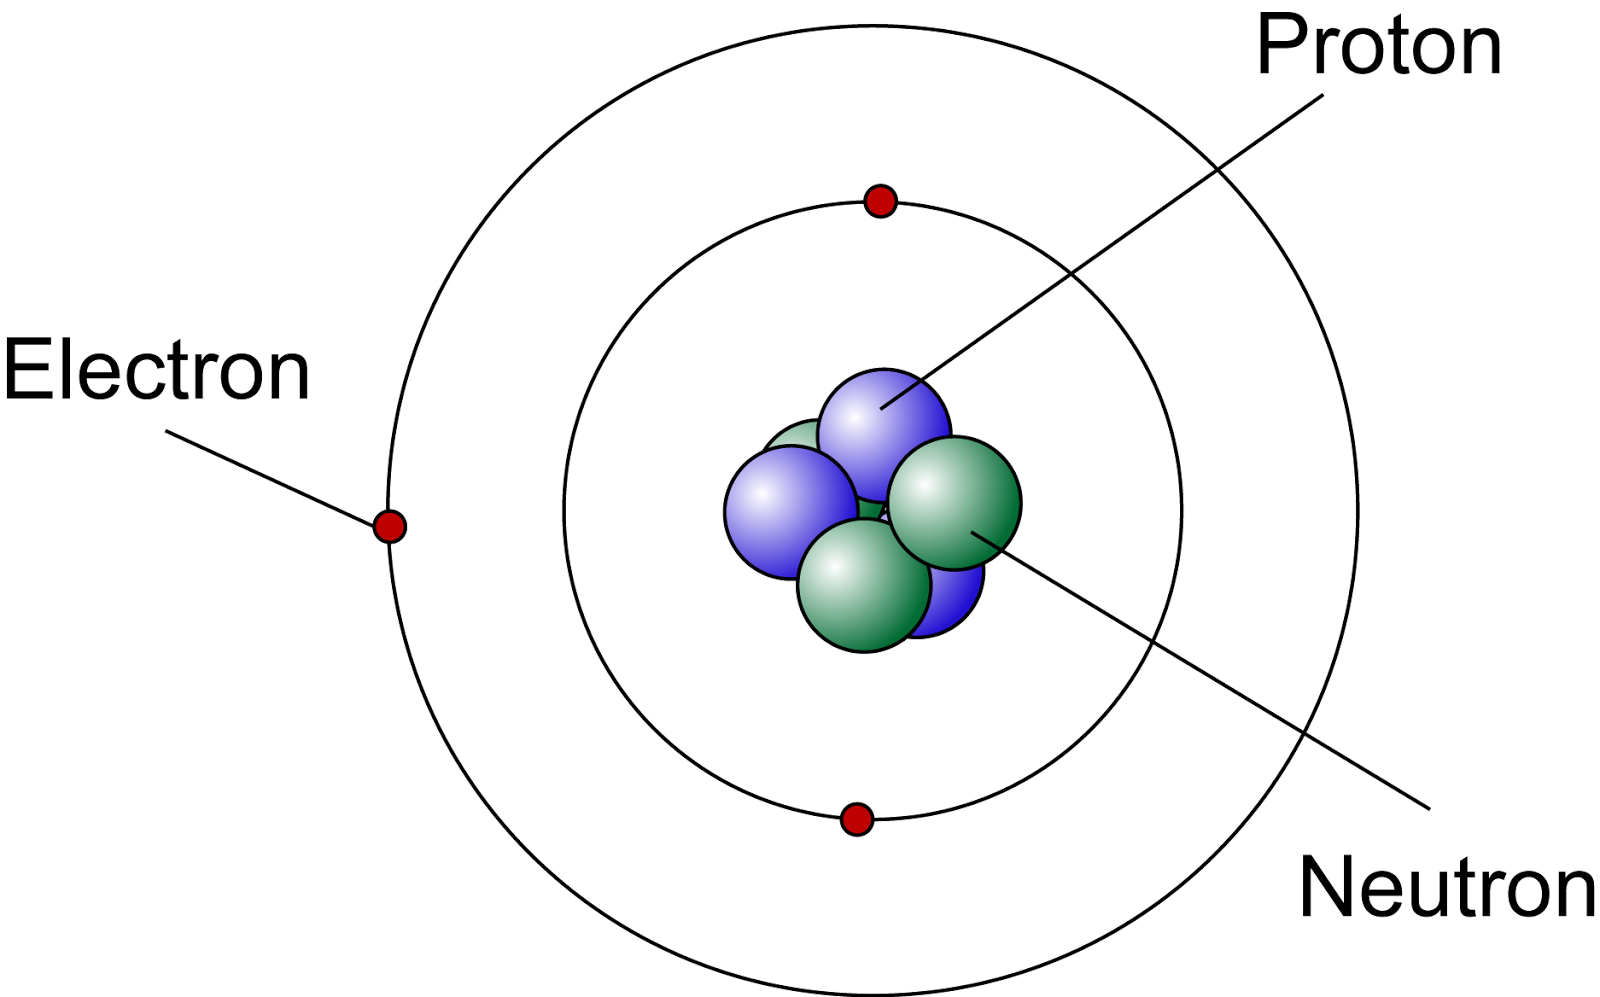
\includegraphics[width=\textwidth]{atom_model}
	\caption{Chadwick's Model of an Atom}
\end{figure}

\subsection{Subatomic Particles}

\begin{defn}
Atoms are comprised of smaller fundamental particles known as subatomic particles. The three core subatomic particles are \textbf{Protons, Neutrons, and Electrons}.

\begin{itemize}
\item Protons have a positive charge and weigh slightly less (but effectively equal to) a Neutron.
\item Neutrons have no/neutrual charge and weigh the most out of the previous two particles.
\item Electrons have a negative charge and weigh roughly 1800 times less than Protons and Neutrons, with effectively no mass.
\end{itemize}
\end{defn}

\noindent
The atom is split into two key portions, the nucleus and the electron cloud. The nucleus is the small, incredibly dense center of the atom that contains its protons and neutrons (which \textit{always results in a positive charge}), and these protons and neutrons within the nucleus are referred to as \textit{nucleons}. The electron cloud is the large outer region of the atom where the electrons move freely and rapidly throughout the nucleus, \textit{thus always resulting in a negative charge}. It has no firmly defined area for any atom and contains various shell and subshell levels which contain orbitals for the electrons.

\subsubsection{Nuclear Notation}

Nuclear Notation is used to indicate the atomic number and mass number of an atom of isotope, and it is formed by writing an elemental symbol preceded by a subscript indicating its atomic number (Z) and a superscript indicating its mass number (A). \\

\noindent
\note{Together, an atom with a specific atomic number and a specific mass number form a \textbf{nuclide.}}

\begin{figure}[H]
	\centering
	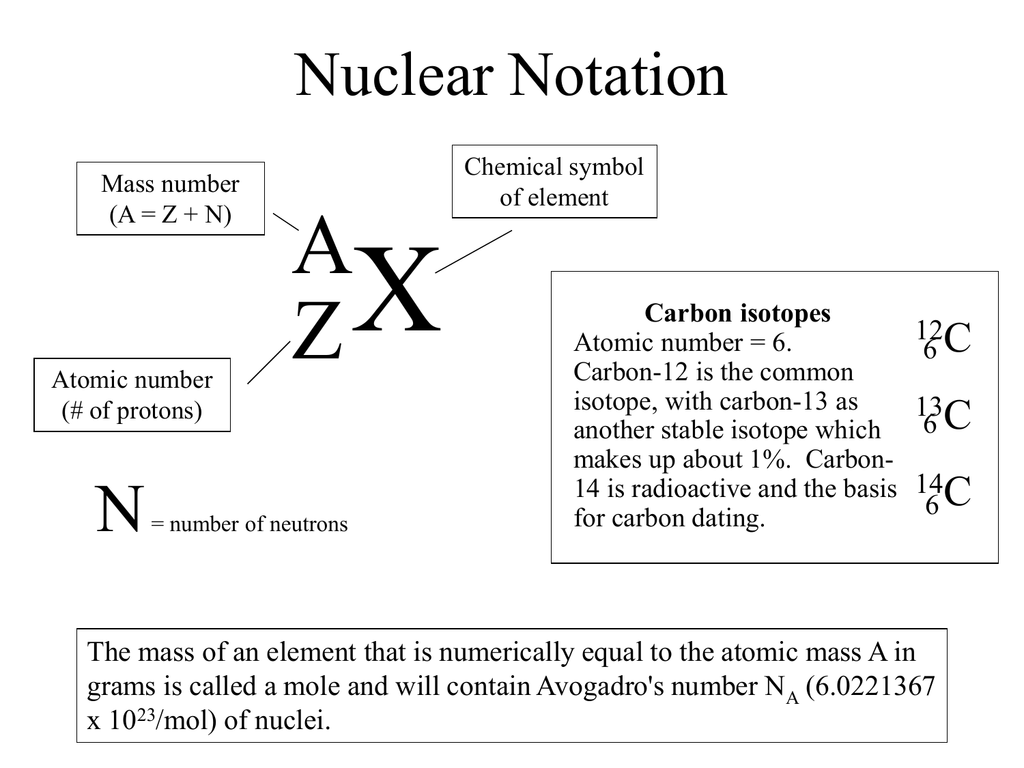
\includegraphics[width=\textwidth]{nuclear_notation}
	\caption{Nuclear Notation Model}
\end{figure}

\begin{defn}
The Atomic Number, denoted by Z, is the number of protons in the nucleus of the atom, and it acts as the primary definition of each type of atom (or Element). Atomic Numbers 1 through 92 (excluding Technetium and Promethium) are naturally occuring and the remaining 93 through 118 are synthetic. \note{As Atoms always hold a neutral charge, the number of electrons will always equal the number of protons and the atomic number.} \\

\noindent
The Mass Number is the sum of the number of protons and neutrons within the nucleus of an atom, and it is a count, \textbf{not} an atomic mass.
\end{defn}

\subsection{Isotopes}

\begin{defn}
Isotopes are atoms of an element that have the same number of protons and electrons but a different number of neutrons, and they are named by denoting the name of the element followed by its newfound mass number (such as Cobalt-60 or Carbon-14).
\end{defn}

\noindent
As an element is determined by the number of protons in the nucleus, the nucleus can have a variable number of neutrons without changing the charge but resulting in changes to the atom's mass number, and this change results in slightly different physical properties but generally similar chemical properties. \\

\noindent
\note{The mass number minus the atomic number is equal to the number of neutrons present in an isotope.}

\subsubsection{Isobars}

\begin{defn}
Isobars are atoms/nuclides of different chemical elements that have the same number of nucleons. Examples include Iron-58 (\ce{^{58}_{26}Fe}) and Nickel-58 (\ce{^{58}_{27}Ni}), or Calcium-40 (\ce{^{40}_{20}Ca}) and Argon-40 (\ce{^{40}_{18}Ar}).
\end{defn}

\subsection{Atomic Mass}

\begin{defn}
The atomic mass is a weighted average that accounts for the number of isotopes for the element, the percent abundance of each isotope, and the relative mass of each isotope (with Carbon-12 as the reference point).
\end{defn}

\section{Lecture 2: Electronic Structure and Chemical Periodicity}

\textbf{References chapter 4, sections 4.4 to 4.7 of the textbook.}

\subsection{The Periodic Table}

\begin{defn}
\textbf{The Periodic Law} \\

\noindent
When elements are arranged in order of increasing atomic number, elements with similar chemical behavior occur at regularly recurring (or \textit{periodic}) intervals.
\end{defn}

\begin{itemize}
\item Period: The horizontal row of elements in the periodic table.
\item Group: The verticle column of elements in the periodic table.
	\begin{itemize}
	\item There are three ways to name the columns: US, EU, and IUPAC
	\item There are four groups with non-numerical names: Alkali Metals, Alkali Earth Metals, Halogens, and Nobel Gases
	\end{itemize}
\item Chemical Periodicity: The variation in properties of elements as a function of their position on the periodic table (or how atoms change as they travel up/down the periodic table).
	\begin{itemize}
	\item There are three properties of elements that exhibit chemical periodicity: metallic vs. non-metallic character, atomic size, and electronegativity.
	\end{itemize}
\end{itemize}

\noindent
\note{Increasing atomic number \textbf{does not} always equal increasing atomic mass.} \\

\noindent
Elements in the periodic table can be classified in one of two ways: either by their electron configurations (nobel gases, representative elements, transition metals, or inner transition/rare earth metals) or their physical properties (metals/non-metals/metalloids)

\subsubsection{Representative Elements}

\begin{defn}
Representative elements are all of the elements located in the first two columns (denoted as the \elvl{s} area) or columns 13-17 (denoted as the \elvl{p} area).
\end{defn}

\noindent
Most elements are representative elements, and they generally have a partially or completely full \elvl{s} electron level and either an empty or partially filled \elvl{p} electron level.

\subsubsection{Alkali Metals (Group IA)}

\begin{itemize}
\item Members: Lithium (Li), Sodium (Na), Potassium (K), Rubidium (Rb), and Cesium (or Caesium) (Cs)
\item They only have one valence electron.
\item All soft, shiny metals.
\item All very reactive with water.
\end{itemize}

\subsubsection{Alkaline Earth Metals (Group IIA)}

\begin{itemize}
\item Members: Beryllium (Be), Magnesium (Mg), Calcium (Ca), Strontium (St), and Barium (Ba)
\item They all have two valence electrons.
\item All soft, shiny metals.
\item Only moderately reactive with water.
\end{itemize}

\subsubsection{Halogens (Group VIIA)}

\begin{itemize}
\item Members: Flourine (F), Chlorine (Cl), Bromine (Br), Iodine (I), and Astatine (At)
\item They all have seven valence electrons.
\item They all exist as diatomic molecules.
\item They are all very reactive colored substances.
\item Almost all are all gases at room temperature (or slightly above room temperature), except for Bromine, which is a liquid at room temperature.
\end{itemize}

\subsubsection{Noble Gases}


\begin{itemize}
\item Members: Helium, Neon, Argon, Krypton, Xenon, and Radon
\item They all have a full valence shell of electrons.
\item They are all completely unreactive (hence the name "Noble," as they are too noble to react with other substances).
\item They are all gases at room temperature.
\end{itemize}

\subsubsection{Transition Element}

\begin{defn}
Transition elements are located in the \elvl{d} area of the periodic table, and their electrons fill the \elvl{D} energy level.
\end{defn}

\subsubsection{Inner Transition Element}

\begin{defn}
Inner Transition Elements are located in the \elvl{f} area of the periodic table, and their electrons fill the \elvl{f} energy level. This series are referred to as \textbf{Lanthanides and Actinides} and are generally known as "Rare Earth Elements."
\end{defn}

\subsection{Physical Properties of Table Elements}

\subsubsection{Metals}

\begin{itemize}
\item Luster (Shine)
\item Thermal Conductivity
\item Electrical Conductivity
\item Malleability (can be rolled into sheets)
\item Ductility (can be drawn into wires)
\item All solids at room temperature (except for Mercury)
\item High Density
\item High Melting Point
\end{itemize}

\noindent
\note{There are 94 actively known metals.}

\subsubsection{Non-Metals}

\noindent
\note{Non-metals are generally characterized by their lack of the properties of \textit{luster, thermal conductivity, electrical conductivity, and malleability} in reference to metals.}

\begin{itemize}
\item Can be solids, liquids, or gases at room temperature.
	\begin{itemize}
	\item Nitrogen (N), Oxygen (O), Hydrogen (H), Chlorine (Cl), Flourine (F), Helium (He), Neon (Ne), Argon (Ar), Krypton (Kr), Xenon (Xe), and Radon (Rn) are all \textbf{gases}.
	\item Carbon (C), Phosphorus (P), Sulfur (S), Selenium (Se), Iodine (I), Astatine (At), and Tellurium (Te) are all \textbf{solids}.
	\item Bromine (Br) is a \textbf{liquid}.
	\end{itemize}
\item Generally have lower density and lower melting points than metals.
\end{itemize}

\subsection{Periodic Table Trends}

\subsubsection{Metallic Character}

\begin{defn}
Metallic character is a general chemical property that describing how `metallic' an element is, and for any given period/row in the periodic table, it increases from right to left, and for any given group, it increases going top to bottom. For example, Sodium (Na) is more Metallic than Magnesium (Mg) but less metallic than Potassium (K).
\end{defn}

\subsubsection{Non-Metallic Character}

\begin{defn}
Non-metallic character is another general chemical property that describes how `non-metallic' an element is (and subsequently, it works in the exact opposite manner to metallic character). As such, for any given period, it increases from left to right, and for any given group, it increases going bottom to top. For example, Chlorine (Cl) is more non-metallic than Phosphorus (P) but less non-metallic than Flourine (F).
\end{defn}

\subsubsection{Metalloids and Semiconductors}

\begin{defn}
Metalloids are an element whose properties intermediate between those of metals and non-metals, and there are eight known metalloids: Boron (B), Sillicon (Si), Germanium (Ge), Arsenic (As), Antimony (Sb), Tellurium (Te), Polonium (Po), and Astatine (At).
\end{defn}

\noindent
\note{Metalloids reside along the stepped line which divides the metals and non-metals.}

\begin{defn}
Semiconductors are metalloids that do not conduct electrical currents at room temperatures but are able to conduct electrical currents at higher temperatures, and there are three main semiconductors: Sillicon (Si), Germanium (Ge), and Antimony (Sb).
\end{defn}

\noindent
\note{Semiconductors are vital in the electronics industry.}

\subsubsection{Atomic Size}

Atomic Radii tend to increase from right to left within any given period and increase from top to bottom for any given group. For example, Helium is rougly the smallest whereas Francium is roughly the largest.

\subsubsection{Electronegativity}

\begin{defn}
Electronegativity is a measure of the relative attraction that an atom has for the shared electrons within its bonds.
\end{defn}

\begin{itemize}
\item The higher the electronegativity of an element, the greater the electon-attracting ability of the atoms of that element.
\item Electronegativity generally increases from left to right within a given period and from bottom to top within a given group.
\item Electronegativity depends on numerous factors: atomic size, nuclear charge, and the number of non-valence electrons.
\end{itemize}

\subsection{Electon Shells, Subshells, and Orbitals}

\subsubsection{Base Review of Electrons}

\begin{itemize}
\item Electrons are the smallest of the three main subatomic particles.
\item Electrons have very small mass.
\item They reside in the electron cloud surrounding the nucleus.
\item Their rapid movement around the nucleus defines the size of the atom.
\item The information regarding the behavior and the arrangements of electrons outside of the nucleus is definved from quantum mechanics.
\item Electrons have spin.
\item Energy in an electron is defined and restricted, so it cannot just go `anywhere.'
\item An energy on electrons is quantized, meaning that it can only have certain values.
\end{itemize}

\subsubsection{Electron Shells}

\begin{defn}
An \textbf{electron shell} is a defined region of space about a nucleus that only contains electrons with approximately the same energy. The \textbf{shell number}, \elvl{n}, is used to identify the electron shell. Electron shells are numbered 1 to 7, and electrons in higher shell numbers have more energy.
\end{defn}

\begin{itemize}
\item Not all electron shells have an equal number of electrons.
\item The number of electrons in a shell generally follows the formula $N = 2n^{2}$, where \elvl{n} is the electron shell level. (I.e., level 3 would have $2(3)^{2}$ or 18 electrons.) 
\item Lower level shells fill before higher ones.
\end{itemize}

\subsubsection{Electron Subshells}

Within an electron shell, there are subshells and orbitals. A subshell is a defined region of space within an electron shell that contains electrons of the same energy level, such as \elvl{s}, \elvl{p}, \elvl{d}, or \elvl{f}.

\begin{itemize}
\item The number of subshells in an electron shell is equal to the shell number.
\item The number of electons in each subshell is defined and independent of the shell number.
\begin{multicols}{2}
	\begin{itemize}
	\item \elvl{s} has 2 electrons.
	\item \elvl{p} has 6 electrons.
	\item \elvl{d} has 10 electrons.
	\item \elvl{f} has 14 electrons.
	\end{itemize}
\end{multicols}
\item Electron subshells are denoted by the electron shell number followed by the letter of the electron subshell with a superscript denoting the number of the number of electrons in the given subshell, such as $1s^{2}$.
\end{itemize}

\subsubsection{Electron Orbitals}

\begin{defn}
Electron orbitals are regions of space within an electron subshell where with a specific energy is most likely to be found.
\end{defn}

\noindent
\note{The number of orbitals in each subshell is one-half of the number of electrons within the subshell, as each orbital can hold two electrons.}

\begin{multicols}{2}
\begin{itemize}
\item \elvl{s} has 1 orbital.
\item \elvl{p} has 3 orbitals.
\item \elvl{d} has 10 orbitals.
\item \elvl{f} has 14 orbitals.
\end{itemize}
\end{multicols}

\subsubsection{The Aufbau Principle}

Electron shells fill according to the \textit{Aufbau Principle}, wherein electrons normally occupy electron subshells in an atom in order of increasing subshell energy, and the energy of subshells can overlap.

\subsection{Electron Configuration}

\begin{defn}
Electron configuration serves as a shorthand notation describing the sbushells in an atom that are occupied by electrons.
\end{defn}

\noindent
Electron configuration is written by starting at the beginning (no electrons) and then continuously filling electron subshells until the correct number of electrons are represented. (Example table below)

\begin{table}[H]
\centering
\begin{tabular}{|c|c|l|}
\hline
Element & Number of Protons (Z) & Electron Configuration \\
\hline
Hydrogen & 1 & $1s^{1}$ \\
\hline
Helium & 2 & $1s^{2}$ \\
\hline
Carbon & 6 & $1s^{2} 2s^{2} 2p^{2}$ \\
\hline
Neon & 10 & $1s^{2} 2s^{2} 2p^{6}$ \\
\hline
Sodium & 11 & $1s^{2} 2s^{2} 2p^{6} 3s^{1}$ \\
\hline
Potassium & 19 & $1s^{2} 2s^{2} 2p^{6} 3s^{2} 3p^{6} 4s^{1}$ \\
\hline
Rubidium & 37 & $1s^{2} 2s^{2} 2p^{6} 3s^{2} 3p^{6} 4s^{2} 3d^{10} 4p^{6} 5s^{1}$ \\
\hline
Cesium & 55 & $1s^{2} 2s^{2} 2p^{6} 3s^{2} 3p^{6} 4s^{2} 3d^{10} 4p^{6} 5s^{2} 4d^{10} 5p^{6} 6s^{1}$ \\
\hline
\end{tabular}
\end{table}

\begin{figure}[H]
	\centering
	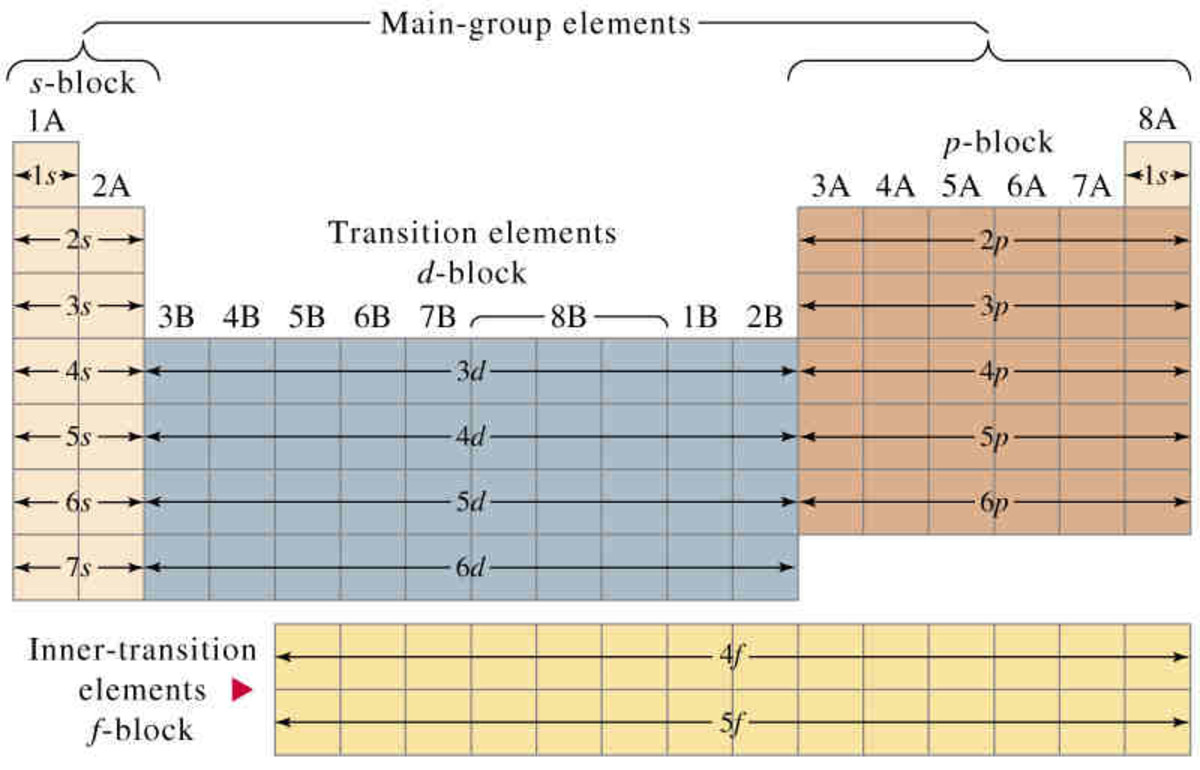
\includegraphics[width=\textwidth]{electron_configuration_table}
	\caption{Ground State Electron Configurations of the Elements}
\end{figure}

\subsubsection{Condensed Electron Configuration}

Electron configuration can also be condensed by utilizing a starting point element (commonly a noble gas) surrounded by brackets then continuing the electron configuration from there. \\

\noindent
For example, as Sodium's electron configuration is $1s^{2} 2s^{2} 2p^{6} 3s^{1}$ and Neon's electron configuration is $1s^{2} 2s^{2} 2p^{6}$, one could condense the electron configuration for Sodium down to [Ne]$3s^{1}$. \\

\noindent
\note{For \elvl{d}, use one less than the period, and for \elvl{f}, use two less than the period.}

\subsection{Paramagnetic and Diamagnetic Substances}

\begin{itemize}
\item Atoms where all electron orbitals are occupied by pairs of electrons are called \textit{diamagnetic} atoms.
\item Atoms where all electron orbits are not occupied by pairs of electrons are called \textit{paramagnetic} atoms.
\end{itemize}

\subsubsection{Visualizing Electron Orbitals}

We can visualize electron orbitals using arrows. Levels that are completely filled are diamagnetic and those that are not are paramagnetic.

\begin{figure}[H]
	\centering
	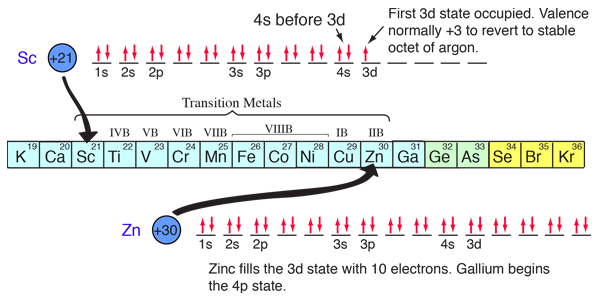
\includegraphics[width=\textwidth]{electron_orbitals_visualization}
	\caption{Electron orbitals visualized with arrows. In this diagram, Scandium (Sc) is paramagnetic and Zinc (Zn) is diamagnetic.}
\end{figure}
